\documentclass[11pt]{article}
\usepackage{tocloft}
\usepackage{graphicx}
\usepackage{calc}
\usepackage{amssymb}
\usepackage{color}
\usepackage{array}
\usepackage[sc]{mathpazo}
\usepackage{url}
\usepackage[final]{pdfpages}

%\linespread{1.05}
\oddsidemargin=0pt
\evensidemargin=0pt
\textwidth=6.5in
\topmargin=0pt
\headheight=0pt
\headsep=0pt
\textheight=9in
% EXPERIMENTAL
%\parindent=0pt
%\parskip=3pt
\setlength{\parindent}{0cm}
\newcommand\secfont{\fontfamily{cmss}\selectfont}%\textwidth 5.5truein
\newcommand\pifheading[1]{{\secfont\textbf{#1}:}}
%\oddsidemargin -0.40truein
%\textheight 8.0truein
%\topmargin -0.25truein
\def\lo{
	\mathrel{\raise.3ex\hbox{$<$}\mkern-14mu\lower0.6ex\hbox{$\sim$}}
}
\def\hi{
	\mathrel{\raise.3ex\hbox{$>$}\mkern-14mu\lower0.6ex\hbox{$\sim$}}
}

\textwidth = 6.6 in
\textheight = 9.1 in
\oddsidemargin = -0.05 in
\evensidemargin = +0.05 in
\topmargin = -.1 in
\headheight = 0.0 in
\headsep = 0.0 in
\parskip = 0.06in
\newcommand\registered{{\ooalign{\hfil\raise .00ex\hbox{\scriptsize R}\hfil\crcr\mathhexbox20D}}}

%% Define a new 'leo' style for the package that will use a smaller font.
\makeatletter
\def\url@leostyle{%
	\@ifundefined{selectfont}{\def\UrlFont{\sf}}{\def\UrlFont{\small\ttfamily}}}
\makeatother
%% Now actually use the newly defined style.
\urlstyle{leostyle}

%\pagestyle{empty}
%\includeonly{previous,proposal_references}
%\includeonly{proposal_references}
%\includeonly{previous}

% TOC

\begin{document}
	\pagenumbering{gobble}
	%%%%%%%%%%%%%%%%%%%%%%%%%%%%%%%%%%%%%%%%%%%%%%%%%%%%%%%%%%%%%%%%%%%%%
	\begin{center}
		\textbf{\Large
			AST101: Our Corner of the Universe \\
			\vspace*{0.1cm}
			Lab 1: Stellarium and The Celestial Sphere
		}
	\end{center}
	
	\vspace*{0.5cm}
	
	\hrule
	{\Large Name:}\vspace*{0.5cm}\\\hrule
	{\Large Lab section:}\vspace*{0.5cm}\\\hrule
	{\Large Group Members:}\vspace*{0.5cm}\\\hrule
	\vspace*{0.5cm}
	
	%%%%%%%%%%%%%%%%%%%%%%%%%%%%%%%%%%%%%%%%%%%%%%%%%%%%%%%%%%%%%%%%%%%%%
	\section{Introduction}
	
	Following the prelab, you should be now acquainted with the basics of how to use Stellarium. Now, we'll use it to take a good look at the basic motions of the sky, and see how the Celestial Sphere model developed. We'll also take an early look at the motion of perhaps the most important object in the entire sky: the Sun!
	
	\subsection*{Materials}
	
	This lab makes extensive use of Stellarium. If you do not have your own computer with Stellarium installed, you may borrow one of the laptops in the classroom from your TA. Do not take this laptop with you! Remember, you're supposed to be working in groups, and not everyone needs to have one.
	
	\subsection*{Objective}
	
	To see with your own eyes the motions of the sky described during the lecture, and to get a better understanding of the concepts described.
	
	\newpage
	
	\section{First Look at the Celestial Sphere}
	
	\subsection{Can You Tell What's Spinning?}
	
	Today, we take it for granted that the Earth moves around the Sun, and that the Earth spins on an axis, creating the apparent motion of the night sky. In short, the Earth does most of the moving. But that wasn't obvious to ancient astronomers. The early Greeks thought that the sky was this grand Celestial Sphere that spun around the Earth, and the objects on the sky were bound to it. The apparent motion of the celestial objects was due mostly to the sphere spinning, as well as the ability for some objects like the Sun to move along the sphere.
	
	\noindent
	\textbf{Question 1.} Before you turn on your computer, let's see how such a mistake could be made. Stand up, and have your group mates stand around you. Then, spin in place. Next, stop spinning, but have everyone in your group move in a circle around you.\\
	
	If you pay attention only to your group mates and not the background behind them, could you easily tell whether you were spinning, or whether they were spinning around you?\\
	\vspace*{1.5cm}
	
	\hrulefill\\
	\noindent
	
	\textbf{Question 2.} Now, boot up Stellarium. Don't worry about the time or location, but turn off the atmosphere so you can 
	see the stars even during the daytime.
	(There is a button along the bottom menu, or use the hotkey A). Now, increase the time speed so that you can actually see the stars move. Looking at the sky, can you tell whether the planet in Stellarium is spinning, or whether the sky is moving around it?\\
	\vspace*{1.5cm}
	
	
	\hrulefill\\
	
	\newpage
	
	% Deleted these questions -- they are awfully easy. Is "where do the stars go during the day" actually hard for them?
	
	
	%\subsection{Stars On The Sphere}
	%
	%\textbf{Question 3.} Turn the atmosphere back on, and set the time to some time during the day. Looking at the sky, what stars, if any, do you see?\\
	%\vspace*{1.5cm}
	%
	%\hrulefill\\
	%
	%\newpage
	%Propose deleting these questions -- they are awfully easy.
	%\textbf{Question 4.} Without changing the time, turn off the atmosphere. Has the number of stars you can see changed with the atmosphere off? \\
	%\vspace*{1.5cm}
	%
	%\hrulefill\\
	%
	%\textbf{Question 5.} Anna and Bob are having a debate about the stars in the Celestial Sphere model:\\
	%
	%\textbf{Anna:} I think only half of the Celestial Sphere has stars, and the other half doesn't. We only see half of the sphere at a time, and at night, the half we see is full of stars, but during the day, the half we see only has the Sun!\\
	%
	%\textbf{Bob:} I don't think that's quite right. I think the whole sphere is full of stars, but during the day, the bright light of the Sun and our atmosphere makes the other stars impossible to see. But they should still be there!\\
	%
	%Who do you think is right, and why?\\
	%\vspace*{1.5cm}
	%
	%% Propose deleting these two questions. Turns out 76W is not 180 degrees away from 76E, and having them do the math would be messy.
	% We can pick this idea up when we do beach balls -- "spin the thing, realize that Madrid was where NYC is five hours ago".
	
	% \hrulefill\\
	
	% \textbf{Question 6.} Set yourself to be in Syracuse New York on September 1 at midnight. Get a good look at the sky (It may help to turn on constellation art and labels). Then, change your location by changing your longitude from being "W $766\circ$ 8' 50.72" " to "E $766\circ$ 8' 50.72", that is, change the W to an E, and change the time from midnight to noon. How does the sky compare?\\
	% \vspace*{1.5cm}
	
	% \hrulefill\\
	
	% \textbf{Question 7.} Stand back to back with on of your lab partners, and both spin in the same direction. Do you see different things? Based on this, why were the skies the same in the previous question?\\
	% \vspace*{1.5cm}
	
%	\hrulefill\\
	
	\section{Motion Of The Stars}
	
	\subsection{Star Paths Of Syracuse}
	
	\textbf{Question 6.} Leaving the atmosphere off, set your location to Syracuse. Point your camera to the east. Are the stars rising or setting in the east? If you can't see them moving, change the rate at which time passes so you can see stars moving slowly in
	the sky.\\
	\vspace*{1.5cm}
	
	\hrulefill\\
	
	
	\textbf{Question 7.} Now, point your camera to the west. Are the stars rising or setting?\\
	\vspace*{1.5cm}
	
	\hrulefill\\   
	
	\textbf{Question 8.} After rising, do the stars go to the northern sky, or the southern sky?\\
	\vspace*{1.5cm}
	
	\hrulefill\\
	
	\textbf{Question 9.} Some stars never rise or set, but instead stay above the horizon the entire day. Such stars are called \textbf{circumpolar} stars. Are there any circumpolar stars in Syracuse? What part of the sky are they in?\\
	\vspace*{1.5cm}
	
	\hrulefill\\
	\newpage
	\textbf{Question 10.} What is at the center of the motion of the circumpolar stars? Does this point have a special name?\\
	\vspace*{1.5cm}
	
	\hrulefill\\
	
	\textbf{Question 11.} Point Stellarium's view back to the north, and line your computer up so that the view matches the real world --
	so that, when you look at your computer screen, you are looking north. Find the star Kochab, and click it to highlight it. ({\it Remember you can hit ctrl-F to search for an object. When using the search, click on the magnifying glass to search for Kochab after typing in its name. Then press T to stop the camera from following it around.)} 
	
	Then, all three people
	in your group should point at the location in the {\it actual} sky where you could find that star. 
	
	Set the rate at which time passes so you can see the stars moving slowly. As the star moves on the computer screen, follow
	its path in the {\it actual} sky with your fingers.
	
	(All three people in your group should share one computer for this)
	
	Then, repeat this process with the star Vega, one of the brightest and hottest stars near us. If you can't see Vega, either wait for it to rise, or use Stellarium's search function to find it. Do the same thing as you did before: Your group
	should follow the path of this star as it moves through the sky, rising and setting and rising again. Where are you pointing when Vega dips below the horizon? 
	
	Finally, do this with the stars Altair and then Sirius. Sirius is the brightest star other than the Sun in our sky; this is because it is very hot and quite close. It has a special role in the mythology of many ancient cultures such as the Egyptians.
	
	For each one, watch it move in Stellarium and, as it does so, trace its path with your finger in the sky. You will notice that these travel mostly in the southern sky; you likely will want to point Stellarium toward the south and then move your computer so you are looking south when you look at it.
	
	
	
	\vspace*{1.5cm}
	
	\hrulefill\\
	
	
	
	\newpage
	
	\textbf{Question 12.} On the diagrams below, sketch the paths of these four stars as viewed from Syracuse. (Label the North Celestial Pole (NCP) first.)
	
	Notice that there are two diagrams: one ``3D perspective'' diagram and one ``flat circular'' diagram, like we used in class. You should draw the paths of the stars in both.
	
	The best way to understand how the stars move is to think about how the motion in the real sky maps onto both ways of diagramming it on paper.
	
	
	
	

	\vspace*{1.5cm}
	
	\begin{center}
		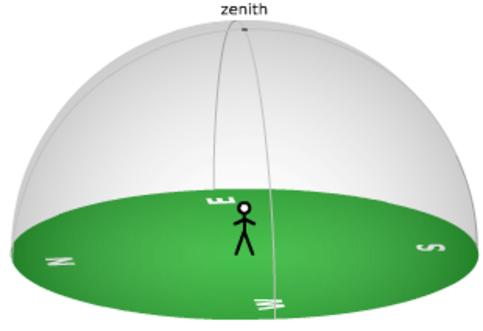
\includegraphics{local_sky}
		
		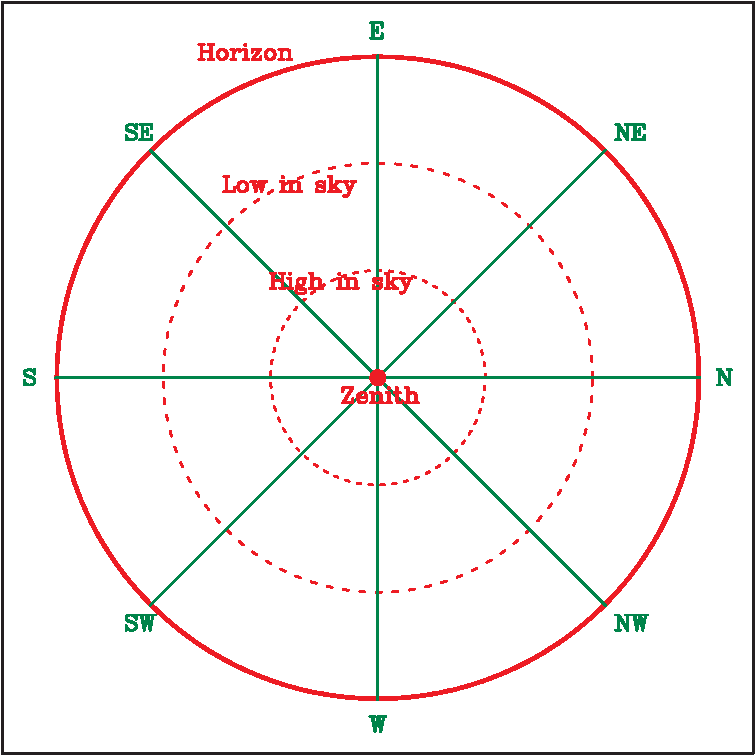
\includegraphics[width=3in]{topsky-crop.pdf}
		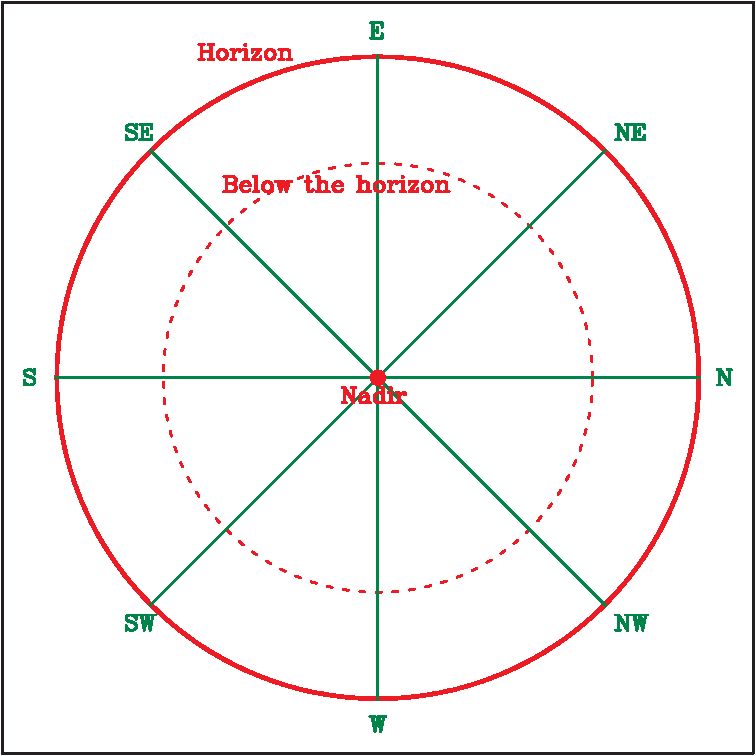
\includegraphics[width=3in]{botsky-crop.pdf}
	\end{center}
	\newpage
	
	\subsection{Stars At The Equator And North Pole}
	
	\textbf{Question 13.} Set your location to the equator (You can either find a location at the equator, or just set the latitude to 0). At the equator, where do the stars rise? Where do they set? \\
	\vspace*{1.2cm}
	
	\hrulefill\\
	
	\textbf{Question 14.} At the equator, is the NCP visible? What about the SCP (South Celestial Pole)? Where can they be found? \\
	\vspace*{1.2cm}
	
	\hrulefill\\
	
	
	\textbf{Question 15.} Sketch the paths of the stars for the equator below. Be sure to include the NCP and SCP if they are visible. (Here you don't need to draw in any particular stars -- just show how stars generally move in the sky.) \\
	\begin{center}
	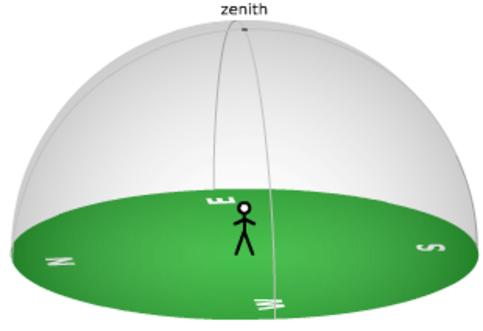
\includegraphics[width=0.45\textwidth]{local_sky}
	
	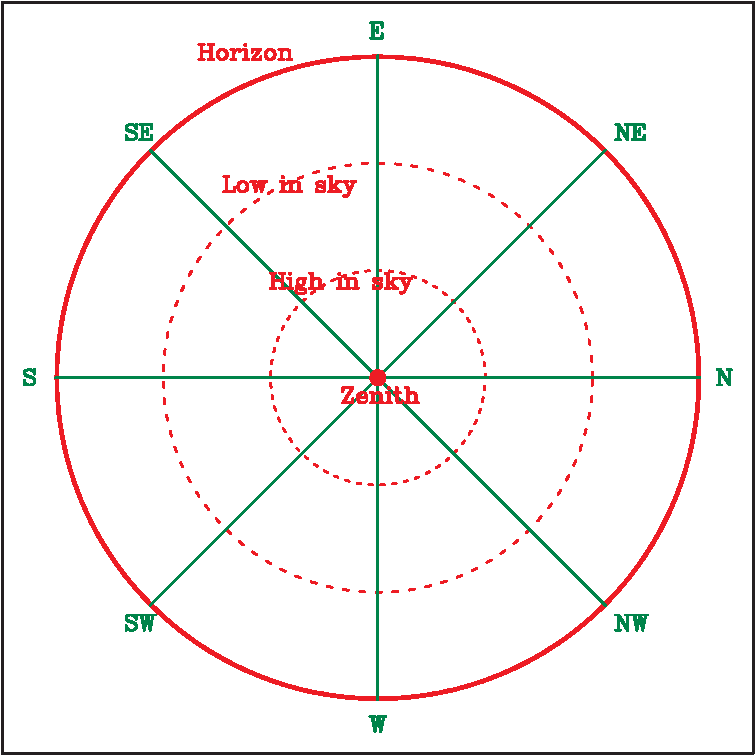
\includegraphics[width=0.4\textwidth]{topsky-crop.pdf}
	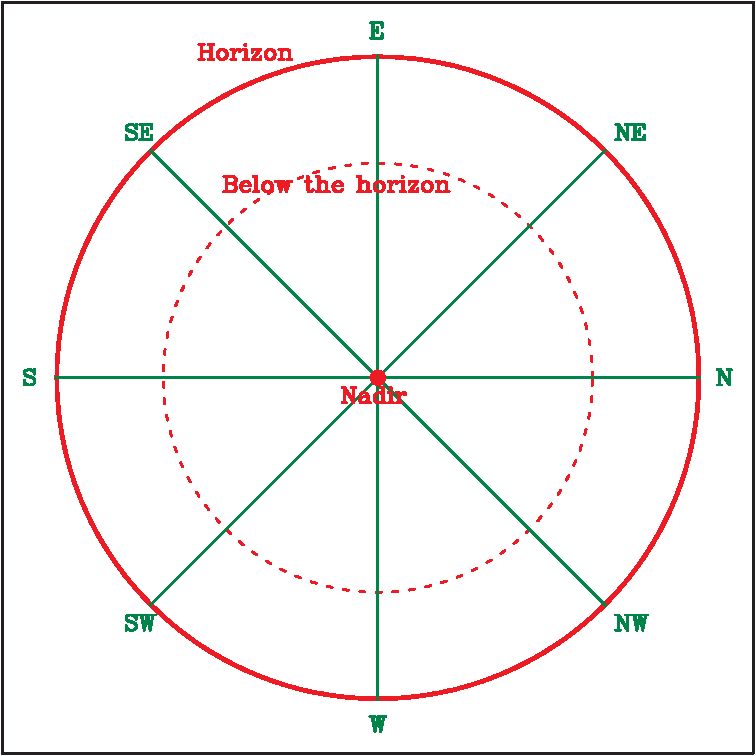
\includegraphics[width=0.4\textwidth]{botsky-crop.pdf}
\end{center}

	\textbf{Question 16.} Set your location to the north pole (latitude of $90^\circ$). Where do the stars rise and set here? Can you see the NCP or SCP?\\
	\vspace*{1.5cm}
	
	\hrulefill\\
	
	\textbf{Question 17.} Sketch the paths of the stars for the north pole below. Be sure to include the NCP and SCP if they are visible. \\
	\vspace*{1.5cm}
		\begin{center}
		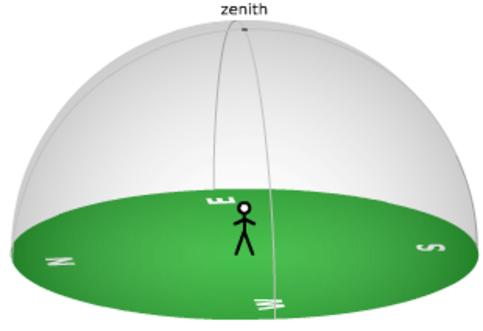
\includegraphics{local_sky}
		
		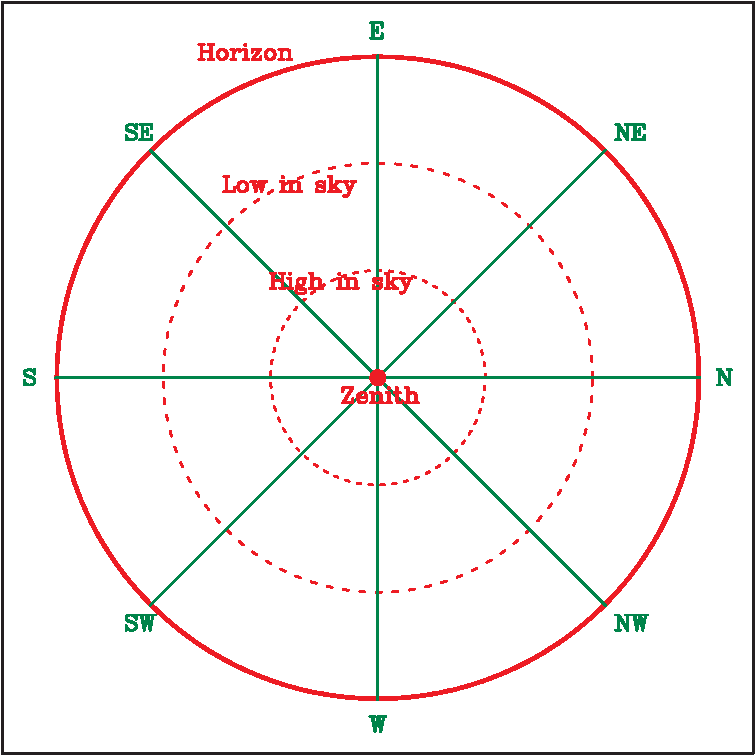
\includegraphics[width=3in]{topsky-crop.pdf}
		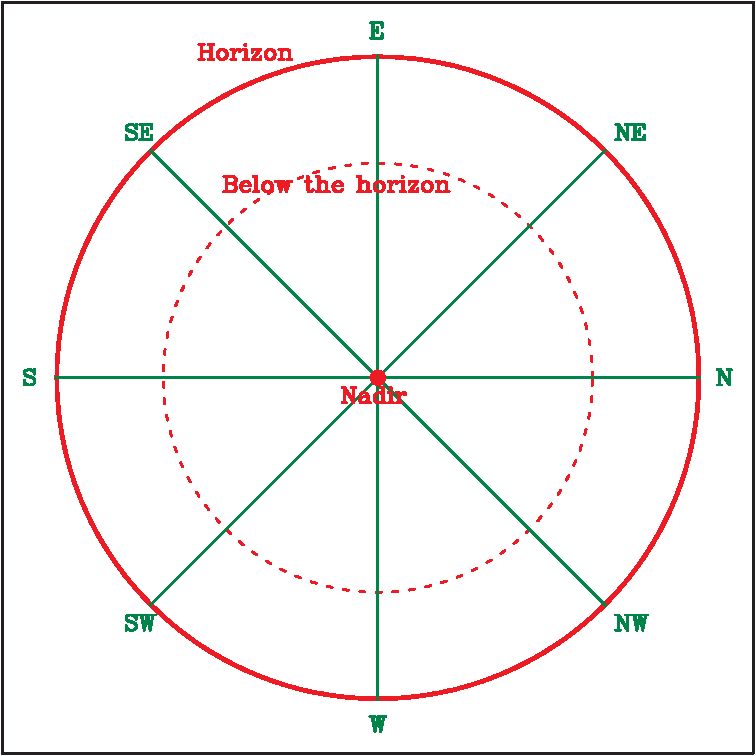
\includegraphics[width=3in]{botsky-crop.pdf}
	\end{center}
	
	
	\newpage
	
	\section{Motion Of The Sun}
	
	{\it (Note: Your TA may ask you to skip sections 4.1 and 4.2.)}
	
	\subsection{Peak Of The Sun}
	
	\textbf{Question 18.} Make sure your location is set to Syracuse New York, and set the time to be 6am on September 21, 2022. Advance time (remember you can speed up time!) until the Sun is at its highest point in the sky; that is, it's at its highest point from the ground. When the Sun is at its highest point, where is it (North, South East, etc.)?\\
	\vspace*{1.5cm}
	
	\hrulefill\\
	
	\textbf{Question 19.} Do the same for March 21. Where is the Sun highest in the sky?\\
	\vspace*{1.5cm}
	
	\hrulefill\\
	
	\textbf{Question 20.} With the Sun at its highest point in the sky. advance time forward by 1 solar day (Hotkey is the equals button) many times. Does the Sun's height in the sky stay the same?\\
	\vspace*{1.5cm}
	
	\hrulefill\\
	
	\textbf{Question 21.} Continue adding solar days until the Sun is at its highest point. Around what date does this occur? What is the date for when the Sun is at its lowest point? Are these days special in some other way?\\
	\vspace*{1.5cm}
	
	\hrulefill\\
	
	\newpage
	
	\subsection{The Sun And The Seasons}
	
	\textbf{Question 22.} Reset time back to September 21, 2022. Find when the Sun rises. What time does it rise? Where (Cardinal direction) does the Sun rise?\\
	\vspace*{1.5cm}
	
	\hrulefill\\
	
	\textbf{Question 23.} What time and where does the Sun set on September 21?\\
	\vspace*{1.5cm}
	
	\hrulefill\\
	
	\textbf{Question 24.} What time and where does the Sun rise and set on June 21, 2022?\\
	\vspace*{1.5cm}
	
	\hrulefill\\
	
	\textbf{Question 25.} What time and where does the Sun rise and set on December 21, 2022?\\
	\vspace*{1.5cm}
	
	\hrulefill\\
	
	\textbf{Question 26.} Based on your previous answers, does the Sun rise exactly east every day? If not, what is the trend?\\
	\vspace*{1.5cm}
	
	\hrulefill\\
	
	\newpage
	
	\textbf{Question 27.} Based on your previous answers, how does the length of the day change with the seasons? \\
	\vspace*{1.5cm}
	
	\hrulefill\\
	
	\textbf{Question 28.} Sketch the paths of the Sun for 6/22, 9/22, and 12/22. Be careful how high your draw your paths; does the Sun ever get as high as directly overhead, the point called the \textbf{Zenith}? \\
	\vspace*{1.5cm}
	
	\begin{center}
		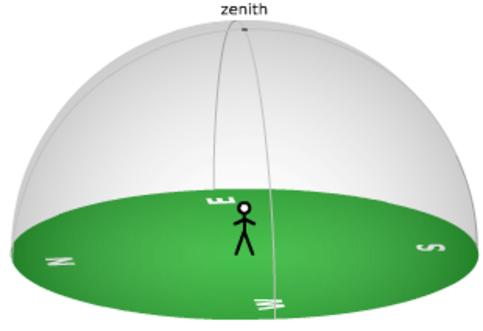
\includegraphics{local_sky}
	\end{center}
	
	\subsection{The Sun And The Zodiac}
	
	\textbf{Question 29.} Reset yourself back to Syracuse New York on September 1, 2022, and put yourself during the day so that you can see the Sun. Turn off the atmosphere, and turn on Constellation Lines and Constellation Labels. What constellation is the Sun in? \\
	\vspace*{1.5cm}
	
	\hrulefill\\
	
	\newpage
	
	\textbf{Question 30.} Speed up the rate of time so that you can see the stars move. Follow the Sun as it moves (you can click on the Sun to select it, then hit the spacebar to follow it); over the course of a single day, does the Sun ever leave the constellation it was in in your previous answer? \\
	\vspace*{1.5cm}
	
	\hrulefill\\
	
	\textbf{Question 31.} Keep allowing time to advance until the Sun is very clearly in a new constellation. About how long did it take the Sun to change constellations? \\
	\vspace*{1.5cm}
	
	\hrulefill\\
	
	\textbf{Question 32.} Your birth sign is the zodiac constellation that was behind the Sun at the time of your birth. Set the time and date to that of your birth as best you know it, and find what constellation was behind the Sun at that time. (If the Sun is below the horizon, advance time until it rises.) Does it match the birth sign your horoscope claims is yours?\\
	\vspace*{1.5cm}
	
	\hrulefill\\
	If you want to know why your birth sign is wrong, look up ``Precession of the Equinoxes'' on Google, or wait until lecture next week!
\end{document}
